% Provenance (never printed): cycle 2 "Questionner le monde de la matiere"
% (solid materials, observing and sorting) and cycle 3 theme 4 (local geology,
% rocks for building); see sources/book1/PROVENANCE.md. Book 1, grade 3, ch. 1.
\chapter{Pedras, seixos e areia}\label{ch:g3:stones-pebbles-sand}

Tom está de férias perto de um \omterm{def:g1:landscapes-around-us:water}{rio}. Na margem de \omterm{def:g3:stones-pebbles-sand:pebble}{cascalho}, onde a água é
rasa, ele pega um \omterm{def:g3:stones-pebbles-sand:pebble}{seixo}. É liso e redondo, quase como um ovo, e cabe na
mão dele. Na semana passada, andando com os pais por uma trilha bem no
alto do mesmo \omterm{def:g1:landscapes-around-us:landform}{vale}, ele viu pedras da mesma cor caídas embaixo de uma
encosta rochosa --- mas aquelas pedras eram pontudas, cheias de arestas e cantos.

Como uma pedra pontuda da \omterm{def:g1:landscapes-around-us:landform}{montanha} virou um \omterm{def:g3:stones-pebbles-sand:pebble}{seixo} liso e redondo lá
embaixo, no \omterm{def:g1:landscapes-around-us:landform}{vale}? Para descobrir, vamos começar pela própria \omterm{def:g3:stones-pebbles-sand:rock}{rocha}.

\begin{omfigure}
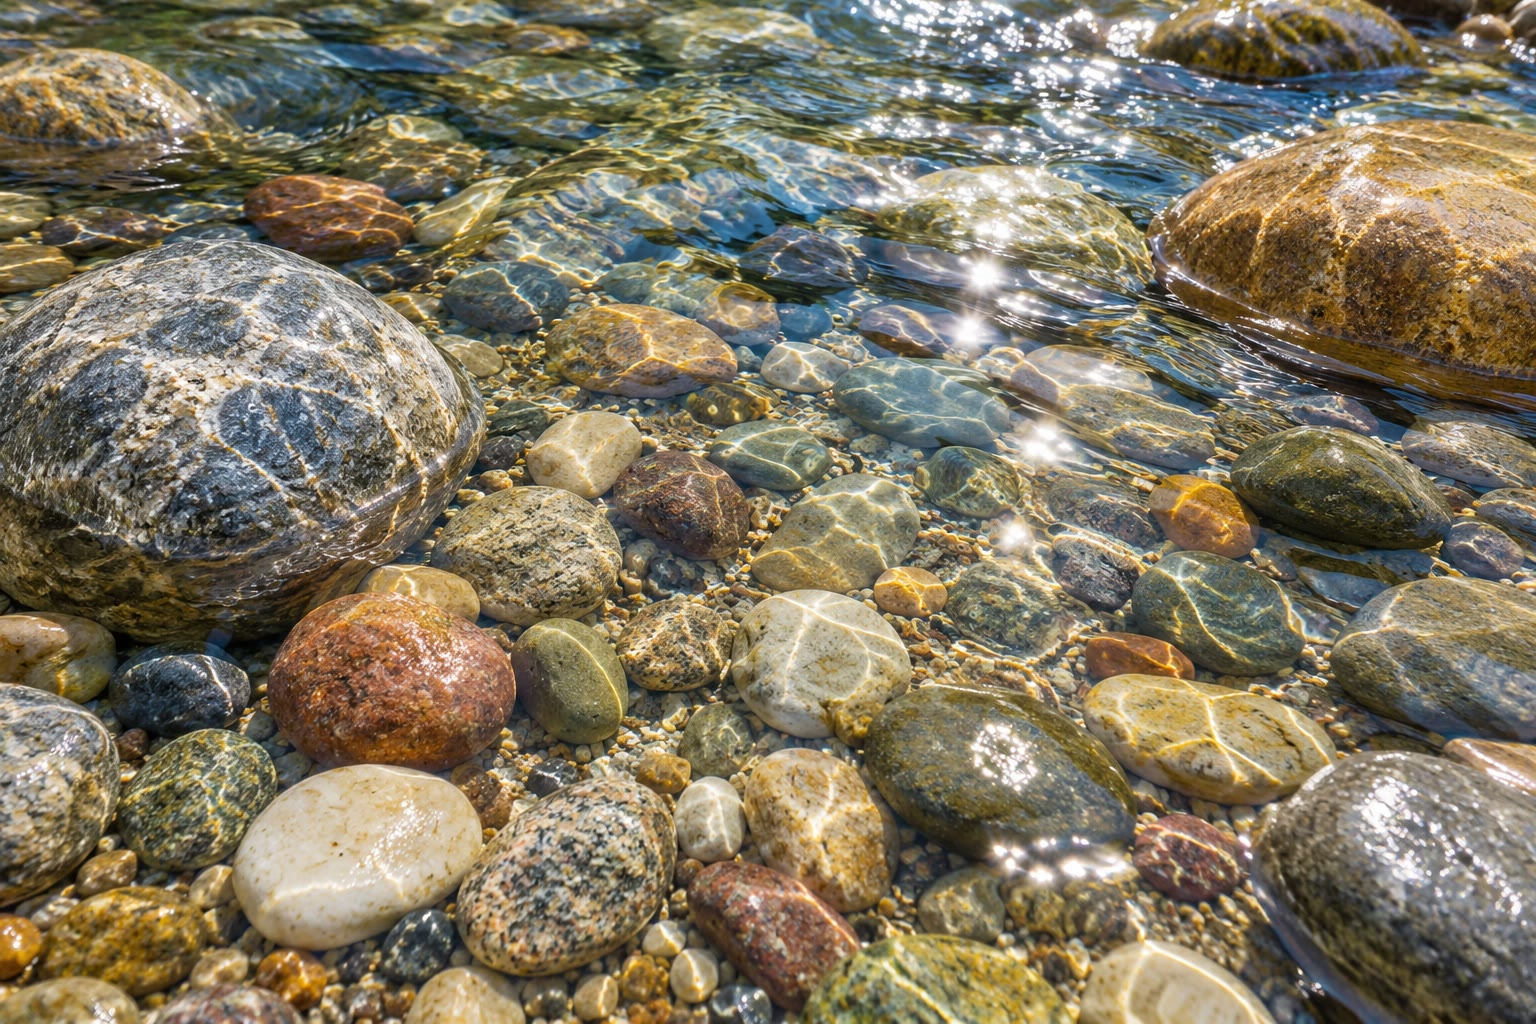
\includegraphics[width=0.62\linewidth]{images/book1/ai/g3-stream-pebbles.jpg}

{\small \omterm{def:g3:stones-pebbles-sand:pebble}{Seixos} redondos sob a água clara de um riacho.}
\end{omfigure}

\begin{recall}
Numa \omterm{def:g1:landscapes-around-us:landscape}{paisagem} há \omterm{def:g1:landscapes-around-us:landform}{montanhas}, \omterm{def:g1:landscapes-around-us:landform}{colinas}, \omterm{def:g1:landscapes-around-us:landform}{vales} e \omterm{def:g1:landscapes-around-us:landform}{planícies}, e \omterm{def:g1:landscapes-around-us:water}{rios} que correm
das terras altas até o \omterm{def:g2:water-on-earth:ocean}{mar} (\cref{ch:g1:landscapes-around-us}). A camada
de cima do chão, onde as plantas crescem, é o solo: os livros de biologia
contam como os seres vivos o formam.
\end{recall}

\section{A rocha: o chão duro sob os nossos pés}

Cave um buraco fundo num jardim. Primeiro você encontra uma terra escura e
fofa, com raízes. Mais embaixo, o solo fica mais claro e cheio de pedras.
E, se você conseguisse cavar bem fundo, sempre chegaria a uma coisa dura
que a pá não consegue cortar: a \omterm{def:g3:stones-pebbles-sand:rock}{rocha}.

\begin{definition}[Rocha e substrato rochoso]\label{def:g3:stones-pebbles-sand:rock}
Uma \emph{rocha}\index{rocha} é um material duro e natural de que a Terra
sólida é feita. O \emph{substrato rochoso}\index{substrato rochoso} é a rocha
maciça que fica embaixo do solo em toda parte nos continentes, e embaixo
da \omterm{def:g3:stones-pebbles-sand:sand}{areia} e da \omterm{def:g3:stones-pebbles-sand:sand}{lama} do fundo do \omterm{def:g2:water-on-earth:ocean}{mar}.
\end{definition}

Na maioria dos lugares, o \omterm{def:g3:stones-pebbles-sand:rock}{substrato rochoso} está escondido pelo solo, pela
grama e pelas árvores. Nós o vemos onde não há solo para cobri-lo: nas
encostas íngremes das \omterm{def:g1:landscapes-around-us:landform}{montanhas}, nos penhascos à \omterm{def:g2:water-on-earth:ocean}{beira-mar} e ao longo das
estradas abertas no meio de uma \omterm{def:g1:landscapes-around-us:landform}{colina}.

\begin{omfigure}
\begin{tikzpicture}[x=1cm, y=1cm, font=\small]
  % bedrock
  \fill[omLithGranite!60] (0,0) rectangle (11,2.2);
  \foreach \x/\y in {0.6/0.5, 1.8/1.4, 3.1/0.7, 4.4/1.6, 5.6/0.4, 6.9/1.2, 8.3/0.6, 9.6/1.5, 10.3/0.4}
    \draw[black!40, line width=0.4pt] (\x,\y) -- ++(0.5,0.25);
  % soil (thick on the left, missing on the steep right)
  \fill[brown!55] (0,2.2) -- (0,3.4) .. controls (2,3.5) and (4,3.4) .. (5.6,3.2) -- (6.4,2.9) -- (6.4,2.2) -- cycle;
  \fill[brown!30] (0,2.2) rectangle (6.4,2.65);
  % rock showing on the right: a hill side with no soil
  \fill[omLithGranite!60] (6.4,2.2) -- (6.4,2.9) -- (7.6,3.9) -- (8.8,4.3) -- (11,4.3) -- (11,2.2) -- cycle;
  \draw[black!60] (0,3.4) .. controls (2,3.5) and (4,3.4) .. (5.6,3.2) -- (6.4,2.9) -- (7.6,3.9) -- (8.8,4.3) -- (11,4.3);
  % grass and roots
  \foreach \x in {0.3,0.8,...,5.3}
    \draw[green!50!black, line width=0.6pt] (\x,{3.4-0.04*\x}) -- ++(0.05,0.18);
  \foreach \x in {1.2,3.4,4.9}
    \draw[brown!80!black, line width=0.5pt] (\x,3.3) -- ++(-0.1,-0.5) -- ++(0.15,-0.3);
  % labels
  \node[anchor=west] at (11.2,3.6) {rocha vista};
  \node[anchor=west] at (11.2,3.2) {na superfície};
  \draw[black!60] (11.15,3.4) -- (9.6,4.15);
  \node[anchor=east] at (-0.2,2.9) {solo};
  \draw[black!60] (-0.15,2.9) -- (0.6,2.9);
  \node[anchor=west] at (11.2,1.1) {substrato rochoso};
  \draw[black!60] (11.15,1.1) -- (10.6,1.1);
\end{tikzpicture}

{\small Um corte no chão. Embaixo do solo há sempre o \omterm{def:g3:stones-pebbles-sand:rock}{substrato rochoso}
maciço. Na encosta íngreme da \omterm{def:g1:landscapes-around-us:landform}{colina}, à direita, falta o solo e a \omterm{def:g3:stones-pebbles-sand:rock}{rocha}
aparece na superfície.}
\label{fig:g3:stones-pebbles-sand:ground}
\end{omfigure}

\section{Da rocha aos seixos}

A \omterm{def:g3:stones-pebbles-sand:rock}{rocha} é dura, mas não dura para sempre. No inverno, a água entra nas
rachaduras de uma \omterm{def:g3:stones-pebbles-sand:rock}{rocha}, congela, incha e alarga as rachaduras. As raízes
também crescem dentro das rachaduras. Pouco a pouco, pedaços se soltam e
caem: é daí que vêm as pedras pontudas embaixo das encostas das \omterm{def:g1:landscapes-around-us:landform}{montanhas}.

Quando uma pedra pontuda cai num riacho da \omterm{def:g1:landscapes-around-us:landform}{montanha}, a água a faz rolar
pelo fundo, bate com ela em outras pedras e a arrasta sobre a \omterm{def:g3:stones-pebbles-sand:sand}{areia}. Os
cantos são os primeiros a se gastar. Quanto mais longe ela viaja, mais
redonda e lisa fica. Quando chega à parte baixa do \omterm{def:g1:landscapes-around-us:landform}{vale}, ela já virou um
\omterm{def:g3:stones-pebbles-sand:pebble}{seixo}.

\begin{definition}[Seixo e cascalho]\label{def:g3:stones-pebbles-sand:pebble}
Um \emph{seixo}\index{seixo} é um pedacinho de \omterm{def:g3:stones-pebbles-sand:rock}{rocha} que foi arredondado e
alisado pela água que o fez rolar, num \omterm{def:g1:landscapes-around-us:water}{rio} ou numa praia. O
\emph{cascalho}\index{cascalho} é um monte de pedrinhas e seixos juntos, com
grãos maiores que os grãos de \omterm{def:g3:stones-pebbles-sand:sand}{areia}.
\end{definition}

\begin{omfigure}
\begin{tikzpicture}[x=1cm, y=1cm, font=\small]
  \draw[ocBlue!70!black, line width=1.2pt, -{Stealth[length=3mm]}] (0,0) -- (12.2,0);
  \node[below, font=\scriptsize] at (6.1,-0.15) {o riacho leva a pedra morro abaixo, um pouco mais longe a cada cheia};
  \foreach \x/\shape/\t in {
     0.8/{(-0.55,-0.1) -- (-0.2,0.5) -- (0.35,0.55) -- (0.6,0.05) -- (0.3,-0.45) -- (-0.35,-0.5) -- cycle}/caída da rocha,
     4.0/{(-0.5,-0.1) [rounded corners=4pt] -- (-0.2,0.45) -- (0.3,0.5) -- (0.55,0.05) -- (0.3,-0.4) -- (-0.35,-0.45) -- cycle}/cantos gastos,
     7.2/{(-0.45,-0.05) [rounded corners=8pt] -- (-0.15,0.42) -- (0.3,0.45) -- (0.5,0.05) -- (0.3,-0.35) -- (-0.3,-0.4) -- cycle}/mais redonda e menor,
     10.4/{(0,0) ellipse (0.45 and 0.3)}/um seixo liso} {
    \begin{scope}[shift={(\x,1.1)}]
      \fill[omLithGranite!80, draw=black!70] \shape;
    \end{scope}
    \node[font=\scriptsize] at (\x,0.35) {\t};
  }
\end{tikzpicture}

{\small A viagem de uma pedra num \omterm{def:g1:landscapes-around-us:water}{rio}: pontuda quando cai da \omterm{def:g3:stones-pebbles-sand:rock}{rocha}, redonda
e lisa depois de um longo passeio \omterm{def:g1:landscapes-around-us:water}{rio} abaixo.}
\label{fig:g3:stones-pebbles-sand:journey}
\end{omfigure}

\begin{remark}[Ler a forma de uma pedra]\label{rem:g3:stones-pebbles-sand:shape}
A forma de uma pedra conta a sua história. Uma pedra pontuda não viajou
para longe da \omterm{def:g3:stones-pebbles-sand:rock}{rocha} de onde se soltou. Um \omterm{def:g3:stones-pebbles-sand:pebble}{seixo} redondo e liso foi rolado
pela água durante muito tempo, num \omterm{def:g1:landscapes-around-us:water}{rio} ou pelas ondas do \omterm{def:g2:water-on-earth:ocean}{mar}.
\end{remark}

\section{A areia e a lama}

As pedras e os \omterm{def:g3:stones-pebbles-sand:pebble}{seixos} que batem uns nos outros também soltam pedacinhos
minúsculos. Depois de muito, muito tempo, esses pedacinhos viram \omterm{def:g3:stones-pebbles-sand:sand}{areia}.
Olhe a \omterm{def:g3:stones-pebbles-sand:sand}{areia} com uma lupa: cada grão é um pedacinho de \omterm{def:g3:stones-pebbles-sand:rock}{rocha}, ou de
concha, muitas vezes arredondado também.

\begin{definition}[Areia e lama]\label{def:g3:stones-pebbles-sand:sand}
% ledger: usgs:wentworth
A \emph{areia}\index{areia} é feita de grãos soltos de \omterm{def:g3:stones-pebbles-sand:rock}{rocha} quebrada, com
menos de 2 milímetros: ainda conseguimos ver cada grão. A \emph{lama}\index{lama}
é feita de grãos tão pequenos que não conseguimos vê-los um por um;
molhada, ela é mole e grudenta.
\end{definition}

Os geólogos classificam os pedaços de \omterm{def:g3:stones-pebbles-sand:rock}{rocha} quebrada pelo tamanho, do maior
ao menor: matacões, \omterm{def:g3:stones-pebbles-sand:pebble}{seixos} e \omterm{def:g3:stones-pebbles-sand:pebble}{cascalho}, \omterm{def:g3:stones-pebbles-sand:sand}{areia} e \omterm{def:g3:stones-pebbles-sand:sand}{lama}.

\begin{omfigure}
\begin{tikzpicture}[x=1mm, y=1mm, font=\small]
  % true size: 1 unit = 1 mm
  \draw[black!40] (0,-14) -- (150,-14);
  \foreach \x in {0,10,...,150} \draw[black!40] (\x,-14) -- (\x,-12.5);
  \foreach \x in {0,50,100,150} \node[font=\scriptsize, below] at (\x,-14.5) {\pgfmathparse{int(\x/10)}\pgfmathresult\,cm};
  % mud: too small
  \node[font=\scriptsize, align=center] at (6,14) {lama};
  \fill[brown!60] (6,0) circle (0.05);
  \node[font=\scriptsize, align=center] at (6,4.5) {grãos pequenos\\demais para ver};
  % sand grains: up to 2 mm
  \node[font=\scriptsize] at (28,14) {areia};
  \foreach \x/\r in {22/0.3, 25/0.5, 28/0.75, 32/1.0}
    \fill[yellow!60!brown, draw=black!50, line width=0.2pt] (\x,0) circle (\r);
  \node[font=\scriptsize, align=center] at (28,5) {menos de\\2 milímetros};
  % gravel and pebbles
  \node[font=\scriptsize] at (78,22) {cascalho e seixos};
  \fill[omLithGranite!80, draw=black!60] (52,0) ellipse (2 and 1.5);
  \fill[black!25, draw=black!60] (62,0) ellipse (4 and 3);
  \fill[omLithGranite!80, draw=black!60] (78,0) ellipse (8 and 6);
  \fill[black!30, draw=black!60] (104,0) ellipse (15 and 10);
  % boulder: off scale
  \node[font=\scriptsize] at (138,22) {matacão};
  \fill[black!20, draw=black!60] (128,-10) .. controls (127,8) and (135,16) .. (142,15) .. controls (150,14) and (152,4) .. (149,-10) -- cycle;
  \node[font=\scriptsize, align=center, fill=white, fill opacity=0.7, text opacity=1, inner sep=1pt] at (139,4) {desenhado bem\\menor que o real};
\end{tikzpicture}

{\small Grãos de \omterm{def:g3:stones-pebbles-sand:rock}{rocha} quebrada, do menor ao maior. A \omterm{def:g3:stones-pebbles-sand:sand}{lama}, a \omterm{def:g3:stones-pebbles-sand:sand}{areia}, o
\omterm{def:g3:stones-pebbles-sand:pebble}{cascalho} e os \omterm{def:g3:stones-pebbles-sand:pebble}{seixos} estão desenhados no tamanho real: compare com uma
régua. Um matacão pode ser do tamanho de uma cadeira, ou de uma casa.}
\label{fig:g3:stones-pebbles-sand:sizes}
\end{omfigure}

\begin{omfigure}
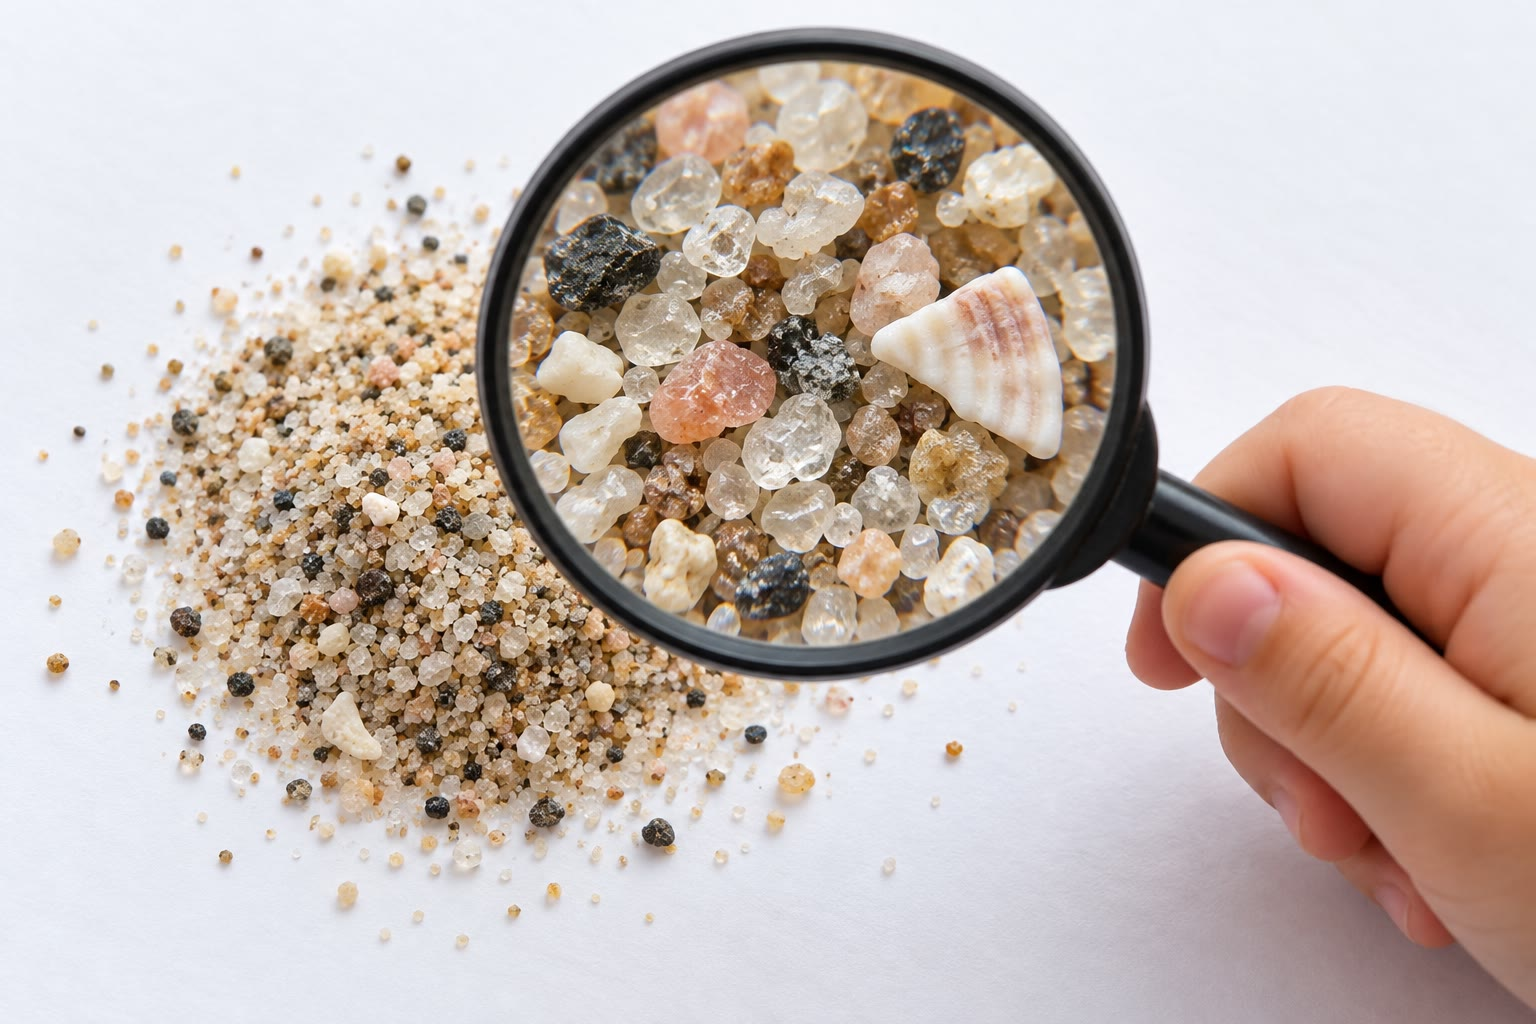
\includegraphics[width=0.55\linewidth]{images/book1/ai/g3-sand-magnifier.jpg}

{\small \omterm{def:g3:stones-pebbles-sand:sand}{Areia} de praia vista com uma lupa: grãos minúsculos de \omterm{def:g3:stones-pebbles-sand:rock}{rocha} e
pedacinhos de concha.}
\end{omfigure}

\begin{method}[Classificar a rocha quebrada pelo tamanho]\label{met:g3:stones-pebbles-sand:sort}
Para dar nome a um pedaço de \omterm{def:g3:stones-pebbles-sand:rock}{rocha} quebrada, observe o tamanho dele:
\begin{enumerate}
  \item se você não consegue ver os grãos, nem bem de perto, é \omterm{def:g3:stones-pebbles-sand:sand}{lama};
  \item se você vê cada grão, mas cada um tem menos de 2 milímetros (a
        espessura de uma moeda), é \omterm{def:g3:stones-pebbles-sand:sand}{areia};
  \item se os pedaços são maiores que isso, mas cabem na sua mão, são
        \omterm{def:g3:stones-pebbles-sand:pebble}{cascalho} e \omterm{def:g3:stones-pebbles-sand:pebble}{seixos};
  \item se um pedaço é pesado demais para levantar, é um matacão.
\end{enumerate}
\end{method}

\begin{example}[Onde encontramos cada tamanho?]\label{ex:g3:stones-pebbles-sand:where}
A água rápida consegue carregar pedras grandes; a água lenta as deixa cair
e só carrega grãos pequenos. Por isso, os matacões e as pedras pontudas
ficam nos riachos íngremes das \omterm{def:g1:landscapes-around-us:landform}{montanhas}; os \omterm{def:g3:stones-pebbles-sand:pebble}{seixos} e o \omterm{def:g3:stones-pebbles-sand:pebble}{cascalho}, nas
margens do \omterm{def:g1:landscapes-around-us:water}{rio} no \omterm{def:g1:landscapes-around-us:landform}{vale}; a \omterm{def:g3:stones-pebbles-sand:sand}{areia} se junta nas praias e nas curvas calmas do
\omterm{def:g1:landscapes-around-us:water}{rio}; e a \omterm{def:g3:stones-pebbles-sand:sand}{lama} se deposita onde a água está quase parada, nas lagoas, nos
\omterm{def:g1:landscapes-around-us:water}{lagos} e na foz dos \omterm{def:g1:landscapes-around-us:water}{rios}.
\end{example}

\section{Rochas duras e rochas moles}

Nem todas as \omterm{def:g3:stones-pebbles-sand:rock}{rochas} são igualmente duras. Algumas, como o granito, são tão
duras que riscam o vidro e duram milhares de anos num muro. Outras se
esfarelam na mão, como o giz, que deixa uma marca branca na lousa. Algumas
\omterm{def:g3:stones-pebbles-sand:rock}{rochas} são feitas de grãos que conseguimos ver; outras são lisas e parecem
iguais de um lado ao outro.

\begin{example}[Três rochas comparadas]\label{ex:g3:stones-pebbles-sand:three}
O \emph{granito} é salpicado de grãos cor-de-rosa, brancos e pretos, e é
muito duro. O \emph{arenito} é feito de grãos de \omterm{def:g3:stones-pebbles-sand:sand}{areia} grudados uns nos
outros; esfregado com o dedo, às vezes ele solta alguns grãos. O
\emph{giz} é uma \omterm{def:g3:stones-pebbles-sand:rock}{rocha} branca, mole e que vira pó. Num ano mais adiante
você vai aprender como cada uma delas se formou.
\end{example}

\begin{omfigure}
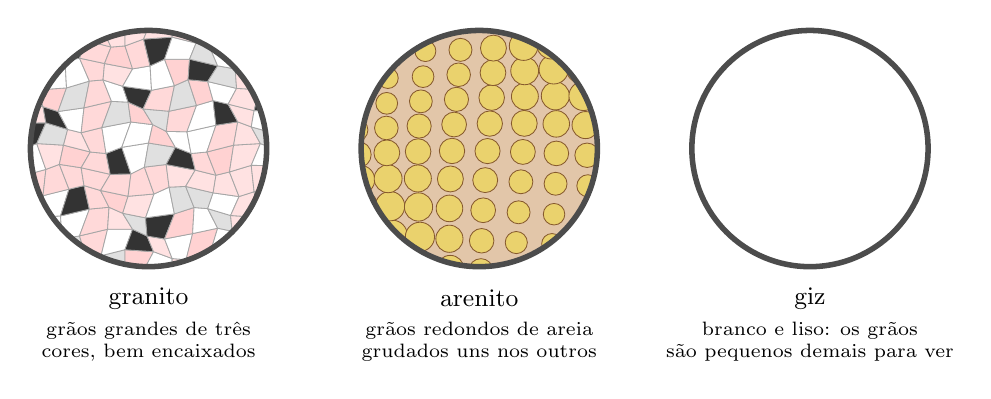
\begin{tikzpicture}[font=\small]
  % three stones seen through a magnifying glass (drawn, not to scale)
  % granite: interlocking grains of three colours
  \begin{scope}
    \clip (0,0) circle (1.5);
    % a jittered lattice: the cells tile the disk with no gap, like the
    % interlocking crystals of granite
    \foreach \i in {-6,...,5} \foreach \j in {-6,...,5} {
      \pgfmathtruncatemacro{\c}{mod(abs(37*\i+17*\j+\i*\j),7)}
      \ifcase\c \def\col{pink!70}\or\def\col{pink!45}\or\def\col{white}\or
        \def\col{black!12}\or\def\col{white}\or\def\col{black!80}\else\def\col{pink!60}\fi
      \fill[\col, draw=black!35, line width=0.3pt]
        ({0.27*\i+0.07*sin(90*\i+131*\j)},{0.27*\j+0.07*cos(77*\i+61*\j)}) --
        ({0.27*(\i+1)+0.07*sin(90*(\i+1)+131*\j)},{0.27*\j+0.07*cos(77*(\i+1)+61*\j)}) --
        ({0.27*(\i+1)+0.07*sin(90*(\i+1)+131*(\j+1))},{0.27*(\j+1)+0.07*cos(77*(\i+1)+61*(\j+1))}) --
        ({0.27*\i+0.07*sin(90*\i+131*(\j+1))},{0.27*(\j+1)+0.07*cos(77*\i+61*(\j+1))}) -- cycle;
    }
  \end{scope}
  \draw[black!70, line width=2pt] (0,0) circle (1.5);
  \node at (0,-1.9) {granito};
  \node[font=\scriptsize, align=center] at (0,-2.45) {grãos grandes de três\\cores, bem encaixados};
  % sandstone: rounded grains touching
  \begin{scope}[xshift=4.2cm]
    \clip (0,0) circle (1.5);
    \fill[brown!45] (-1.6,-1.6) rectangle (1.6,1.6);
    \foreach \x in {-1.5,-1.1,...,1.6} \foreach \y in {-1.5,-1.15,...,1.6}
      \fill[yellow!50!brown!70, draw=brown!70!black, line width=0.3pt]
        ({\x+0.08*sin(97*\x+61*\y)},{\y+0.07*cos(53*\x-89*\y)}) circle ({0.16+0.03*sin(71*\x*\y)});
  \end{scope}
  \draw[black!70, line width=2pt] (4.2,0) circle (1.5);
  \node at (4.2,-1.9) {arenito};
  \node[font=\scriptsize, align=center] at (4.2,-2.45) {grãos redondos de areia\\grudados uns nos outros};
  % chalk: smooth, no grains to see
  \begin{scope}[xshift=8.4cm]
    \fill[white] (0,0) circle (1.5);
  \end{scope}
  \draw[black!70, line width=2pt] (8.4,0) circle (1.5);
  \node at (8.4,-1.9) {giz};
  \node[font=\scriptsize, align=center] at (8.4,-2.45) {branco e liso: os grãos\\são pequenos demais para ver};
\end{tikzpicture}

{\small Três \omterm{def:g3:stones-pebbles-sand:rock}{rochas} vistas com uma lupa (desenho). Os grãos do granito e do
arenito podem ser vistos; o giz parece igual em toda parte.}
\label{fig:g3:stones-pebbles-sand:magnified}
\end{omfigure}

\begin{method}[Observar uma pedra de perto]\label{met:g3:stones-pebbles-sand:look}
Para descrever uma pedra, olhe para ela e toque nela, sem quebrá-la:
\begin{enumerate}
  \item a sua cor, ou as suas cores;
  \item a sua forma: pontuda, com cantos, ou redonda e lisa;
  \item os seus grãos: dá para vê-los? São todos iguais, ou de várias
        cores?
  \item a sensação ao tocá-la: dura, ou mole a ponto de deixar uma marca no papel?
\end{enumerate}
Anote o que você vê numa tabela, com uma linha para cada pedra.
\end{method}

\begin{example}[Uma tabela de três pedras]\label{ex:g3:stones-pebbles-sand:table}
Mia descreve três pedras de uma caixa da escola.
\begin{center}\small
\begin{tabular}{llll}
\hline
Pedra & Cor & Forma & Grãos \\
\hline
A & rosa, branca e preta & redonda & grandes, de três cores \\
B & marrom-amarelada & pontuda & pequenos, todos iguais \\
C & branca & pontuda & nenhum visível \\
\hline
\end{tabular}
\end{center}
A pedra C também deixa uma marca branca no papel. Pelo exemplo acima, a
pedra A parece granito, a pedra B parece arenito e a pedra C parece giz. A
pedra A é redonda: a água a fez rolar durante muito tempo.
\end{example}

\section{As pedras com que construímos}

Há milhares de anos, as pessoas constroem com a \omterm{def:g3:stones-pebbles-sand:rock}{rocha} que encontram por
perto. Nas vilas antigas de uma região, os muros muitas vezes têm todos a
mesma cor, porque foram construídos com a pedra da \omterm{def:g1:landscapes-around-us:landform}{colina} mais próxima.

\begin{definition}[Pedra de construção]\label{def:g3:stones-pebbles-sand:building-stone}
Uma \emph{pedra de construção}\index{pedra de construcao@pedra de construção} é uma \omterm{def:g3:stones-pebbles-sand:rock}{rocha} cortada ou
moldada para construir muros, telhados, degraus, pontes ou calçamentos.
\end{definition}

Cada \omterm{def:g3:stones-pebbles-sand:rock}{rocha} serve para alguma coisa. O granito, que é duro, dá muros,
degraus e meios-fios que duram séculos. Algumas \omterm{def:g3:stones-pebbles-sand:rock}{rochas}, como a ardósia, se
partem em placas finas e planas: colocadas umas sobre as outras, elas
formam telhados que não deixam a chuva entrar. O arenito e o calcário são
moles o bastante para serem cortados em blocos bem certinhos.

\begin{omfigure}
\begin{minipage}[b]{0.49\linewidth}\centering
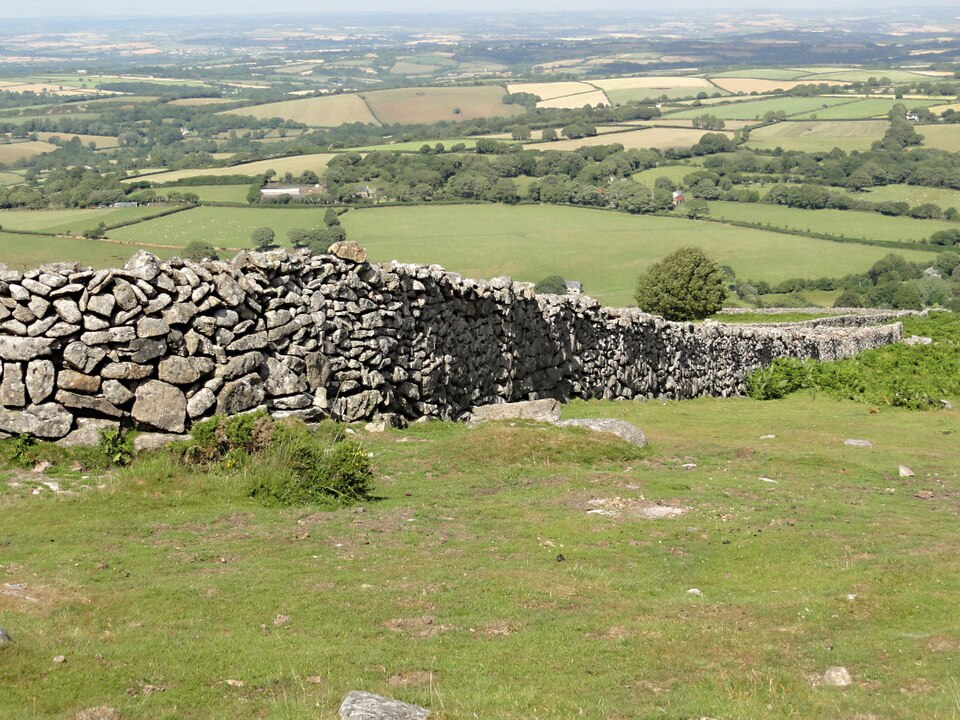
\includegraphics[width=\linewidth]{images/book1/g3-granite-wall.jpg}

{\small Um muro de blocos de granito, construído sem argamassa. Foto: Tony
Atkin, Geograph (CC BY-SA 2.0).}
\end{minipage}\hfill
\begin{minipage}[b]{0.49\linewidth}\centering
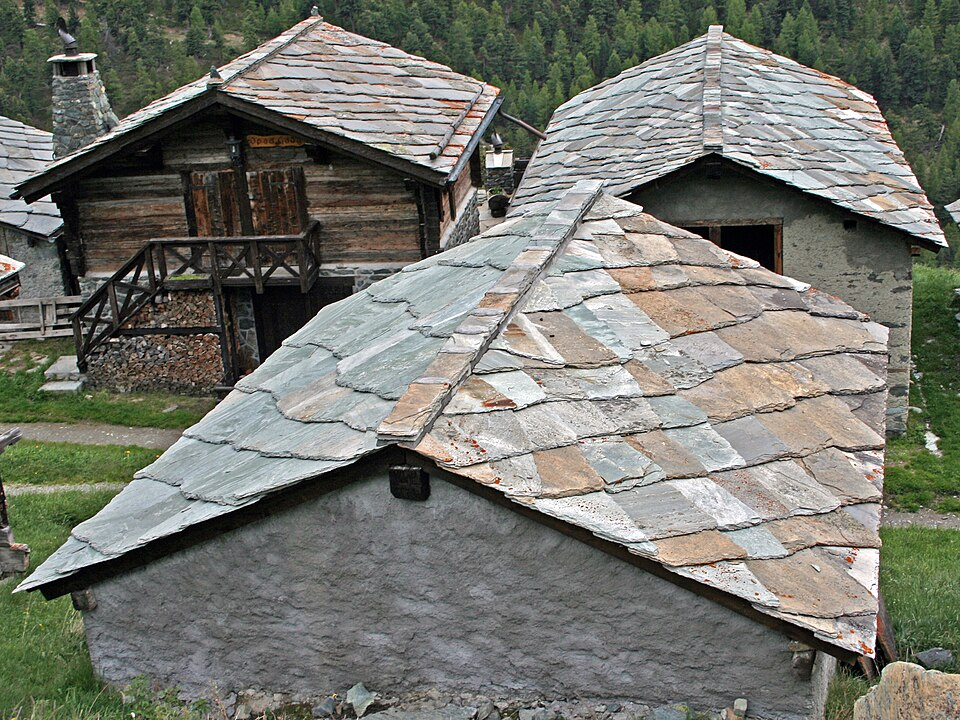
\includegraphics[width=\linewidth]{images/book1/g3-slate-roof.jpg}

{\small Telhados de lajes de pedra finas e planas numa vila de \omterm{def:g1:landscapes-around-us:landform}{montanha} da
Suíça. Foto: Michael C. Rygel (CC BY-SA 3.0).}
\end{minipage}
\end{omfigure}

\begin{omfigure}
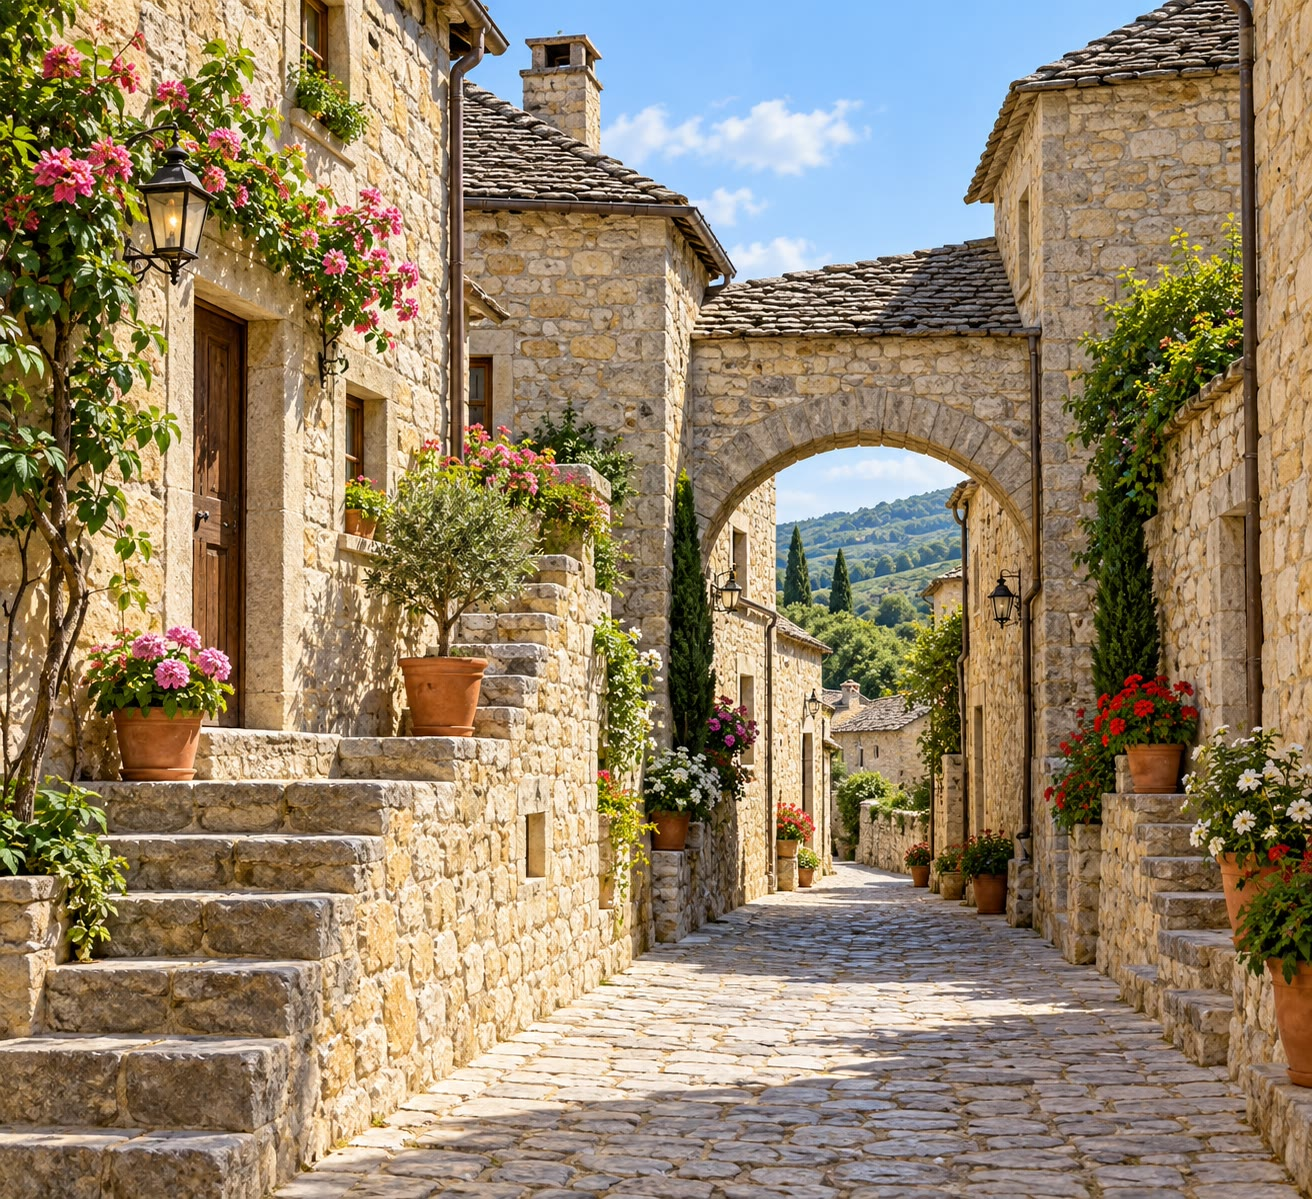
\includegraphics[width=0.6\linewidth]{images/book1/ai/g3-stone-village.jpg}

{\small Uma vila antiga construída toda com a pedra da \omterm{def:g1:landscapes-around-us:landform}{colina} vizinha.}
\end{omfigure}

Hoje também construímos com tijolos, concreto e vidro. Mas o tijolo é feito
de argila cozida, o concreto é feito de \omterm{def:g3:stones-pebbles-sand:sand}{areia}, \omterm{def:g3:stones-pebbles-sand:pebble}{cascalho} e cimento, e o
vidro é feito de \omterm{def:g3:stones-pebbles-sand:sand}{areia}: todos eles também vêm das \omterm{def:g3:stones-pebbles-sand:rock}{rochas} da Terra.

\section{Exercícios}

\begin{exercise}[$\star$]\label{exo:g3:stones-pebbles-sand:1}
O que é o \omterm{def:g3:stones-pebbles-sand:rock}{substrato rochoso}? Onde podemos vê-lo sem cavar?
\end{exercise}

\begin{exercise}[$\star$]\label{exo:g3:stones-pebbles-sand:2}
Coloque em ordem de tamanho, do menor para o maior: \omterm{def:g3:stones-pebbles-sand:pebble}{seixo}, \omterm{def:g3:stones-pebbles-sand:sand}{lama}, matacão,
\omterm{def:g3:stones-pebbles-sand:sand}{areia}.
\end{exercise}

\begin{exercise}[$\star$]\label{exo:g3:stones-pebbles-sand:3}
Um grão mede 1 milímetro. É \omterm{def:g3:stones-pebbles-sand:sand}{areia} ou \omterm{def:g3:stones-pebbles-sand:pebble}{cascalho}? Outro grão mede
3 milímetros: \omterm{def:g3:stones-pebbles-sand:sand}{areia} ou \omterm{def:g3:stones-pebbles-sand:pebble}{cascalho}?
\end{exercise}

\begin{exercise}[$\star$]\label{exo:g3:stones-pebbles-sand:4}
Natural ou feito pelas pessoas? Um \omterm{def:g3:stones-pebbles-sand:pebble}{seixo}; um tijolo; um bloco de granito;
uma placa de vidro; a \omterm{def:g3:stones-pebbles-sand:sand}{areia} de uma praia.
\end{exercise}

\begin{exercise}[$\star$]\label{exo:g3:stones-pebbles-sand:5}
Por que um \omterm{def:g3:stones-pebbles-sand:pebble}{seixo} de \omterm{def:g1:landscapes-around-us:water}{rio} não tem cantos pontudos?
\end{exercise}

\begin{exercise}[$\star$]\label{exo:g3:stones-pebbles-sand:6}
Cite duas \omterm{def:g3:stones-pebbles-sand:building-stone}{pedras de construção} e diga para que cada uma é usada nas fotos
deste capítulo.
\end{exercise}

\begin{exercise}[$\star\star$]\label{exo:g3:stones-pebbles-sand:7}
Tom encontra duas pedras da mesma \omterm{def:g3:stones-pebbles-sand:rock}{rocha}: uma é pontuda, a outra é redonda.
Qual delas viajou mais longe? Explique.
\end{exercise}

\begin{exercise}[$\star\star$]\label{exo:g3:stones-pebbles-sand:8}
No desenho dos tamanhos de grão, quantos centímetros tem o maior \omterm{def:g3:stones-pebbles-sand:pebble}{seixo}?
Quantos grãos de \omterm{def:g3:stones-pebbles-sand:sand}{areia} de 2 milímetros caberiam lado a lado ao longo de
1 centímetro?
\end{exercise}

\begin{exercise}[$\star\star$]\label{exo:g3:stones-pebbles-sand:9}
Onde você esperaria encontrar \omterm{def:g3:stones-pebbles-sand:sand}{lama}: num riacho rápido da \omterm{def:g1:landscapes-around-us:landform}{montanha} ou numa
lagoa calma? Por quê?
\end{exercise}

\begin{exercise}[$\star\star$]\label{exo:g3:stones-pebbles-sand:10}
Os tijolos, o concreto e o vidro são feitos pelas pessoas. Por que ainda
podemos dizer que eles vêm das \omterm{def:g3:stones-pebbles-sand:rock}{rochas} da Terra?
\end{exercise}
